%!TEX encoding = UTF-8 Unicode

\documentclass{essay}
\usepackage[margin=1in]{geometry}
\usepackage[font=small]{caption}
\usepackage{mathtools}

\IfFileExists{config.tex}{\input{config.tex}}

\begin{document}
\sffamily

\setsmallheader{Network-based Measures of Gene Flow}{ECEV 445}{Ansel George}

\section{Introduction}

The evolution of populations is a complex process with strongly entwined
spatial and temporal components. At the local level, individuals compete in
environments that lend to differential reproductive outcomes by means of
natural selection or by random drift on extant variation present across few or
many loci that is generated by mutation and recombination. [citation] At the
spatial level, variation in ecological conditions, such as resource
availability and predation, drive differences in allele frequencies across
space [citation], which over time can lead to formation of subspecies or
speciation events.

These interacting processes are all nonlinear and present complex dynamics that
are analytically intractable and computationally infeasible. Naturally,
researchers must simplify these systems before attempting to study them. One
such process --- gene flow --- describes the transfer of alleles from
from the most part segregated gene pools, or demes, from migrants that move
from one deme to the next. Several broad classes of methods exist for studying
this process, each with strengths and pitfalls, and one class --- network-based
methods --- presents interesting non-parametric strategies for inferring gene
flow.

\begin{figure}
  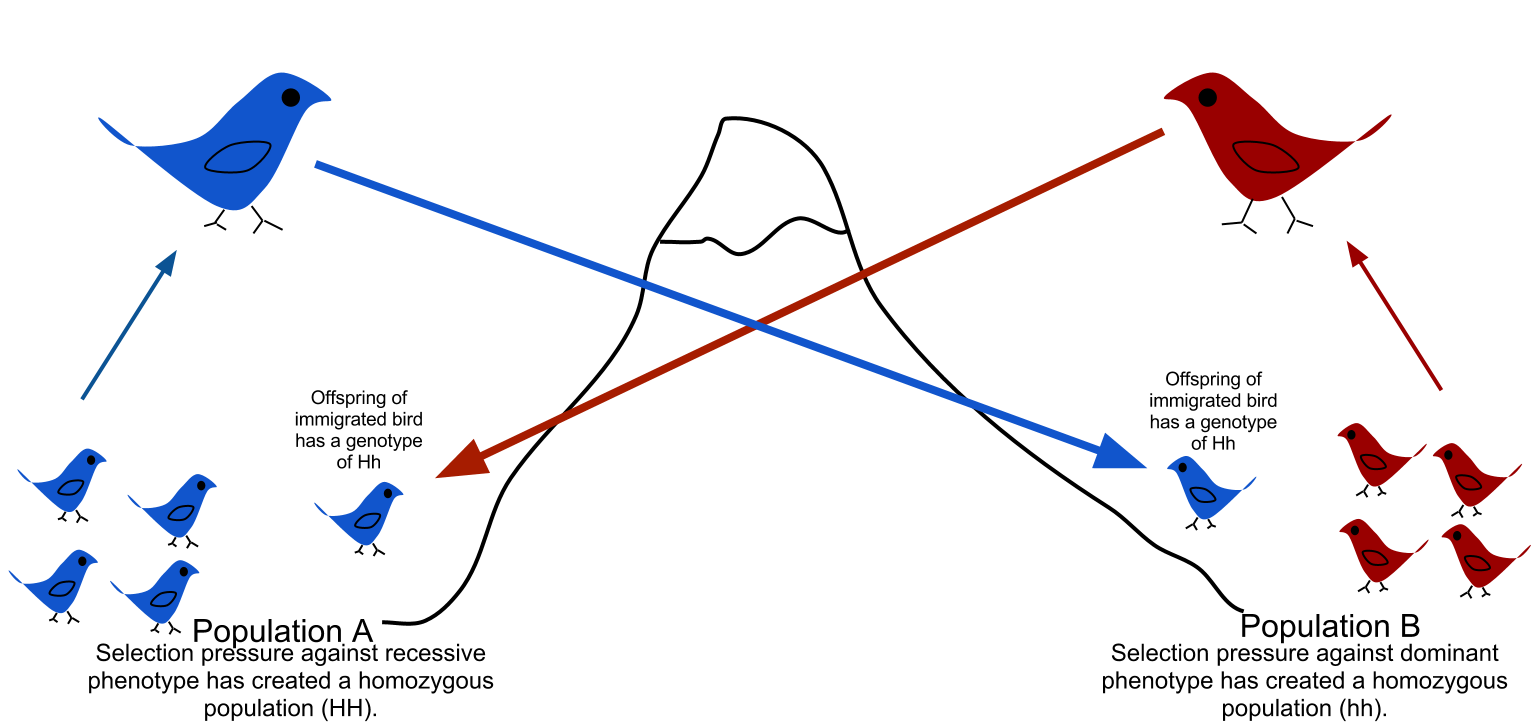
\includegraphics[width=\linewidth]{../Figures/Gene_flow_final.png}
  \caption{By Jessica Krueger --- Own work, CC BY-SA 3.0,
  \url{https://commons.wikimedia.org/w/index.php?curid=19542551}}
\end{figure}

\section{Non-network Methods}

Many methods and strategies exist for inferring gene flow. A brief overview of
several broad classes is presented below. All of these methods involve
computations on genotype data for each individuals, specifically single
nucleotide polymorphisms (SNPs), which are point mutations that are segregating
within or between populations.

\subsection{Bayesian Models}

Several Bayesian approaches to inferring gene flow exist. They derive their
utility from Bayes rule:

\begin{align}
  P(Z, \Theta | X) &\propto P(Z) P(\Theta) P(X|Z,\Theta)
\end{align}

where $Z$ is a set of the subpopulation of origin for each individual, which
may be known or unknown, $\Theta$ is the allele frequency parameters for each
deme, and $X$ is the genotype data.

Many Bayesian approaches exist. They rely on an underlying model where
subpopulations each have a characteristic set of allele frequencies, and given
data, the one computes assignments of individual to source subpopulations and
infers population structure, such as gene flow among them. Various other
simplifying assumptions, such as independence of loci (no linkage), absence of
selection (Hardy-Weinberg equilibrium), are fixed population size
(Wright-Fisher model), are often made to simplify the generative model.

One key method, STRUCTURE~\cite{pritchard_inference_2000}, and its successor,
ADMIXTURE~\cite{falush_inference_nodate}, utilize this approach. Assuming each
individual originates from an unknown number of subpopulations with known
allele frequencies, it uses Markov Chain Monte Carlo (MCMC) and Gibbs sampling
to estimate each parameter by computing likelihoods from the generative model
with a set of estimated parameters and iteratively updating the parameters to
maximize the likelihood. Complementary Bayesian models have also been developed
should allele frequencies be unknown~\cite{corander_bayesian_nodate}.

\begin{figure}
  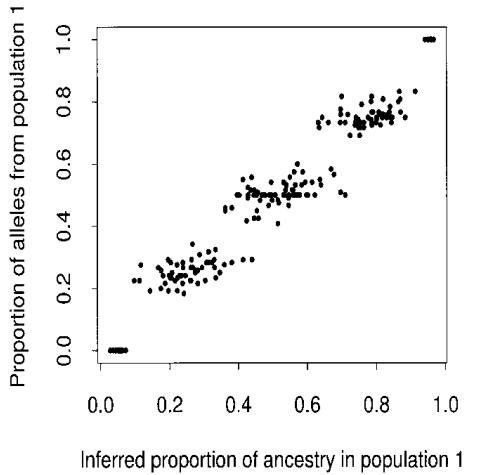
\includegraphics[width=.5\linewidth,keepaspectratio]{../Figures/fig10.png}
  \caption{Clustering results for population of admixed individuals. Each point
  is the estimate from STRUCTURE of the proportion of alleles in an individual
  that originate in a specific population.~\cite{pritchard_inference_2000}}
\end{figure}

This class of methods is capable, depending on the degree of genetic divergence
samples, identifying subpopulations, estimating allele frequencies, and
inferring gene flow among them, but it is most suited for cases where there are
segregating variants particular to each
population~\cite{porras-hurtado_overview_2013}, otherwise the likelihood
function is becomes very flat and optima difficult to find using an MCMC
approach. Because these are Bayesian methods, models can flexible and can
incorporate known information, such as known ancestry and migration patterns,
as priors on the likelihood or as hyperparameters for model parameters.
Increased layers of complexity can introduce new sources of variance, though,
so the deeply nested models are best used when they are shown to improve on
simpler ones.

\subsection{Dimensionality Reduction}

Many techniques exist for multi-dimensional scaling (MDS) that involve linear
and non-linear transformation of data, but for genetic data, the one most
commonly used is principal components analysis (PCA).  Formally, PCA is the
eigenvalue decomposition of the covariance matrix of features and samples:

\begin{align}
  M &= \frac{1}{n-1} X^T X = V \Lambda V^T
\end{align}

where $M$ is the covariance matrix of $X$, $V$ the orthogonal basis for the
eigenspace, and $\Lambda$ the diagonal of the eigenvalues.

Eigenvalues and their corresponding eigenvectors are typically sorted in order
of decreasing magnitude, and per the Eckart-Young theorem, the best
low-dimensional representation of rank $d$ corresponds to the projection of the
data onto the $d$ eigenvectors corresponding to the $d$ largest eigenvalues.

PCA is a simple method that uses linearity and covariance relationships to
tease apart samples based on variation in their features or features based on
variation in the samples. It has many uses in population genetics, and it can
be used to infer gene flow between populations~\cite{mcvean_genealogical_2009}.

\begin{figure}
  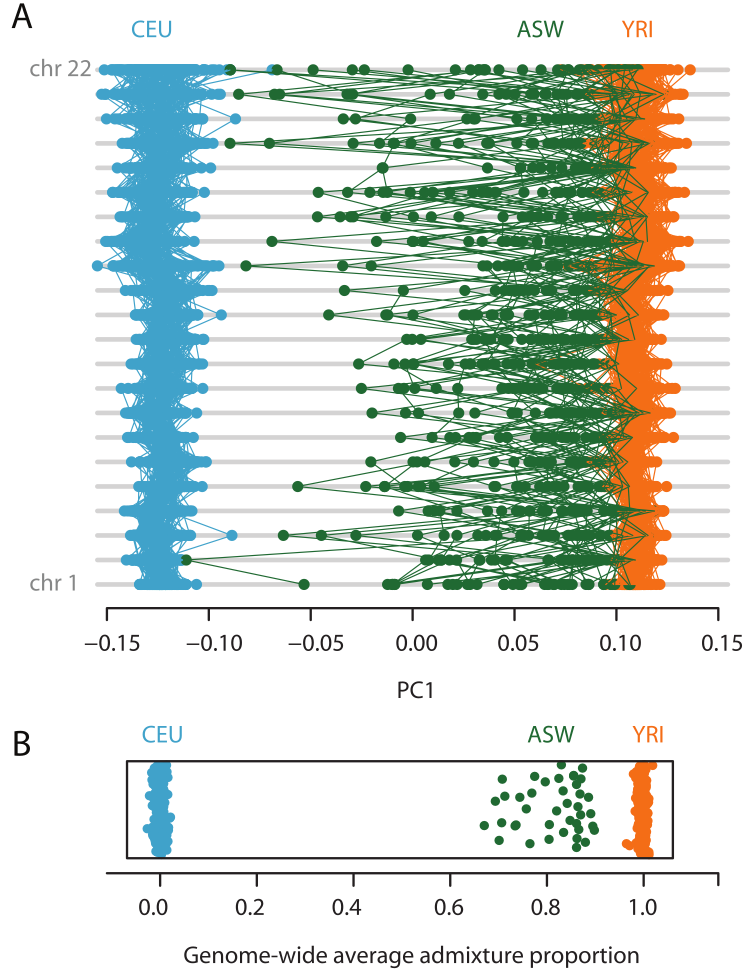
\includegraphics[width=\linewidth,keepaspectratio]{../Figures/fig3.png}
  \caption{Position of admixed individuals (green) along principal
    component axes defined by European (blue) and Yoruban (orange)
    populations~\cite{mcvean_genealogical_2009}.}
\end{figure}

Samples known to originate from different subpopulations will form separate
clusters in principal component space, and individuals admixed from the two
populations will fall somewhere between the two clusters, allowing simple
detection of gene flow.

However, PCA has substantial limitations. Foremost, the principal components
are computed based on all factors that generate variance in samples, which can
include those that don't correspond to gene flow. The proportion of variance
that is directly ascribed to admixture also varies over time, and as the number
of generations after admixture events increases, gene flow is less able to
drive separation along principal components~\cite{mcvean_genealogical_2009}.
This means that PCA is largely ineffective relative to Bayesian- and
model-based methods and, as will be explained below, network-based methods.
Still, the method is computationally fairly simple and does not require
sophisticated software. If the data in question are from recent migrations of
known populations, PCA is adequate.

\begin{figure}
  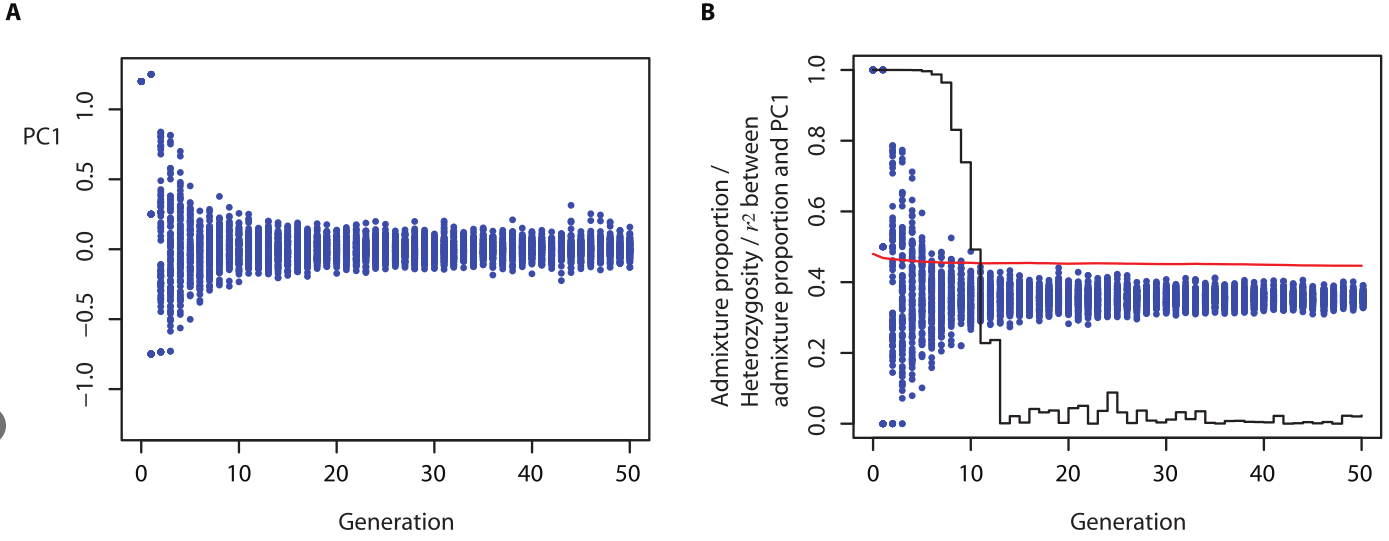
\includegraphics[width=\linewidth,keepaspectratio]{../Figures/fig1a.png}
  \caption{(A) Additionally, the proportion of variance represented in the
    first eigenspace decreases with each generation. (B) The proportion of the
    first principal component that is induced by variation due to admixture
    (black line) decreases over time, bottoming out around $\sim 15$
    generations. This is the case when population heterozygosity is stable (red
    line)~\cite{mcvean_genealogical_2009}.}
\end{figure}

Other pitfalls correspond to the numerical properties of covariances. The
eigenspaces defined by the principal components are themselves a linear
combination of all features or samples. This means that the spatial positioning
of individuals in these spaces are not governed by simple Euclidean distance
relationships. This reduces the interpretability of results beyond obvious
clustering. Lastly, PCA is highly sensitive to outliers and variation in sample
size. Covariances are computed from squares of deviations, so covariances of
outliers are made correspondingly huger. These can lead to spurious distance
relationships between demes.

\begin{figure}
  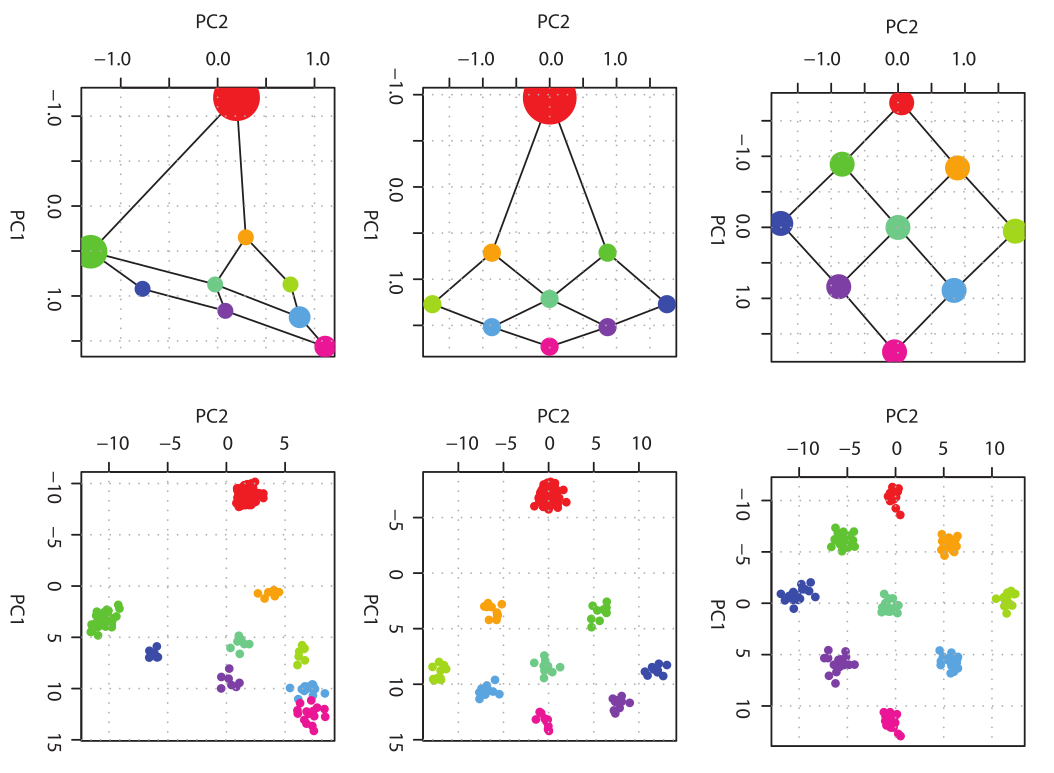
\includegraphics[width=.9\linewidth,keepaspectratio]{../Figures/fig2.png}
  \caption{Principal component distances get skewed by sample size (area of
  dot) for each deme~\cite{mcvean_genealogical_2009}.}
\end{figure}


\section{Network Methods}

Network-based methods as a class differ from those mentioned above in that they
are both non-parametric and information agnostic. The former means that the
methods used to generate genetic network structures do not rely on assumed
prior parameters for some underlying model, and the latter mans that the
information encapsulated by the network structure may be derived from several
underlying evolutionary processes. This does introduce difficulties in terms of
interpretability of results, but it at least creates a visual representation of
subpopulation in terms of the set of characteristics that best separate them.
Several such methods are described below.

\subsection{Population Graph}

The Population Graph is a method for constructing gene flow networks based on
the conditional independence structure for the underlying data samples from
each deme~\cite{dyer_population_2004}. A non-technical description of the
algorithm is as follows:

\begin{enumerate}
  \item Group samples from deme of origin.
  \item Compute genotype centroids for each deme using the samples obtained
    from each.
  \item Generate a distance matrix $D$ containing pairwise genetic distances
    between centroids.
  \item Compute the covariance matrix $\Sigma$ for $D$.
  \item Invert the covariance matrix to obtain the precision matrix ($\Omega =
    \Sigma^{-1}$).
  \item Prune edges connecting demes that are conditionally independent given
    the data.
  \item Generate a network graph from the remaining edges.
\end{enumerate}

The theory behind population graphs is adapted from a method for computing
modularity among different phenotypes and multivariate selection in
populations~\cite{magwene_new_2001}. It produces a graph of genetic similarity
across demes using only edges that contribute the global covariance structure
of the data. More formally, edges are pruned by computing the edge exclusion
deviance~\cite{whittaker_graphical_2009}, defined by:

\begin{align}
  -N\log(1 - \rho^2_{ij|K})
\end{align}

where $N$ is the sample size and $\rho_{ij|K}$ is the correlation between $i$
and $j$ holding all other variables $K$ constant. The deviance follow a
$\chi^2$ distribution with 1 degree of freedom. The goodness of the subsampled
covariance model can be found by computing the model deviance:

\begin{align}
  D &= N \log\frac{| \hat\Sigma |}{| S |}
\end{align}

where model deviance $D$ follows a $\chi^2$ distribution with degrees of
freedom equal to the number of removed edges. $|\hat\Sigma|$ and $|S|$ are the
determinants of the pruned covariance and sample covariance matrices,
respectively.

The precision matrix strategy is formally based on the assumption that data is
generated by a multivariate-Gaussian generative process. Though it can be
extended to describe partial correlations for any underlying distribution, a
multivariate Gaussian process is necessary for claims of conditional
independence in the graph structure to hold. Given that evolutionary processes
involving migration, selection, etc.\ are decidedly non-Gaussian, the goodness of
fit test is necessary for the population graph.

The network structure of the resulting graph is immediately amenable to a
battery of network parameters. Degree and eigenvector centrality of demes
relate to the proportion of migrants in each subpopulation. Shortest path
lengths between nodes relate to coalescent summary $F$ statistics, namely
$F_{st}$~\cite{dyer_population_2004}. Subsets of nodes with high modularity
correspond to interbreeding subpopulations, and degree distributions of the
networks, which in general are consistent with a small-world generative model,
elucidate migratory patterns that can simultaneously be mapped to geographic
characteristics ~\cite{garroway_applications_2008}.

\begin{figure}
  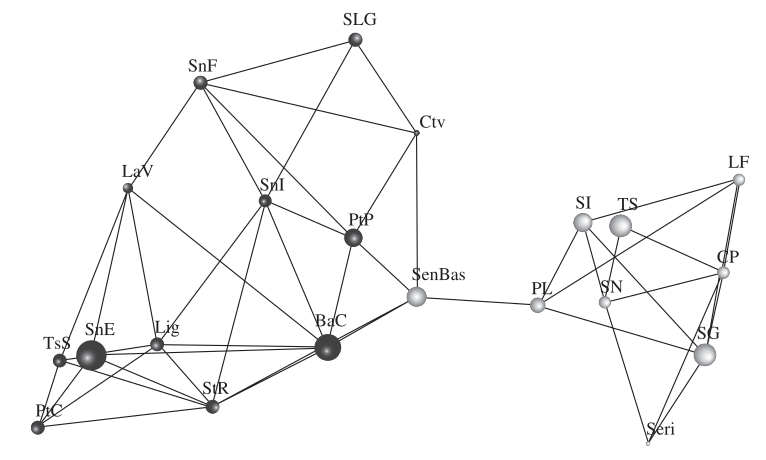
\includegraphics[width=\linewidth,keepaspectratio]{../Figures/fig4.png}
  \caption{Population graph for \textit{L. schottii} dataset~\cite{dyer_population_2004}.}
\end{figure}

Understanding the meaning of the network structure itself requires caution.
The raw covariance graph is itself dense, with each node connected to all
others. Nodes in the population graph with high centrality or low degree do not
necessarily imply the corresponding deme is a critical juncture in terms of
historical population migrations. It should also be noted that genetic `memory'
of historical migrations will persist long after migrations stop, so
connectivity in population graphs need not reflect extant observed migration
patterns.

Interpretation of network properties and metrics must of course be corroborated
by other means. For example, one can compare the population graph with a set of
graphs with demes removed, or one could check that the graph maps to other
relevant details for the population, such as geographical barriers or proximity
to predators. Here, one must take care to avoid issues with multiple-testing
--- regressing network measures against each characteristic from the demes is
likely to yield spurious significant correlations.

This method, though it avoid issues arising arbitrary thresholds to prune
the genetic covariance matrix, requires that the generative process underlying
the data does not strongly deviate from a multivariate Gaussian distribution.
Deme networks that do are not interpretable as population graphs. Additionally,
the computation of precision matrices, which involve computationally expensive
matrix inversions, is impractical for very large samples sizes and is also
numerically unstable.

\subsection{NetView}

NetView is a toolchain that takes genetic data and outputs a graph structure
representing clusters of genetically similar
individuals~\cite{neuditschko_netview:_2012}. It clusters individuals based on
genetic similarity and measures the stability of the clusters to perturbations
of the dataset. Individuals are segregated by pairwise allele sharing distance
(ASD)~\cite{gao_using_2009}, which is demonstrably effective at separating
individuals in other tools, such as PLINK~\cite{purcell_plink:_2007}

NetView relies on a Hamiltonian-based iterative algorithm called Super
Paramagnetic Clustering (SPC) for separating out
subpopulations~\cite{blatt_superparamagnetic_1996}. The technique is
computationally efficient and effective in picking out clusters in data
generated by nonlinear and non-Gaussian processes. Apart from the identity of
clusters, it also is used to compute a `cluster stability' (CS) measure for
each cluster, defined as the range of pairwise distance thresholds at which the
clustering holds. High CS corresponds to strong internal relatedness, and low
CS hints at internal substructure within a given cluster. 

\begin{figure}
  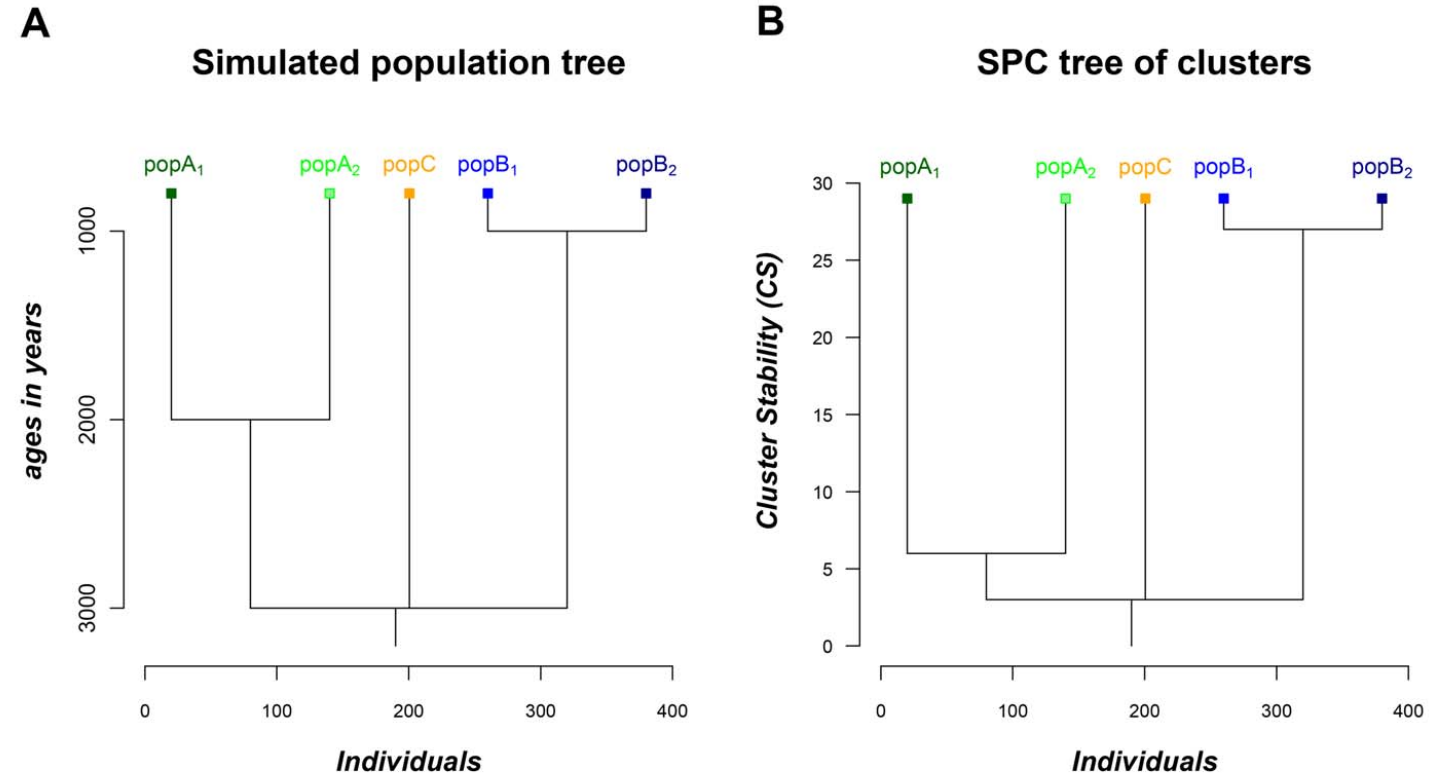
\includegraphics[width=1\linewidth,keepaspectratio]{../Figures/fig6ab.png}
  \caption{Simulated population structure. Strong SPC cluster stability
  corresponds to strong interrelatedness within the
  cluster\cite{neuditschko_netview:_2012}.}
\end{figure}

\begin{figure}
  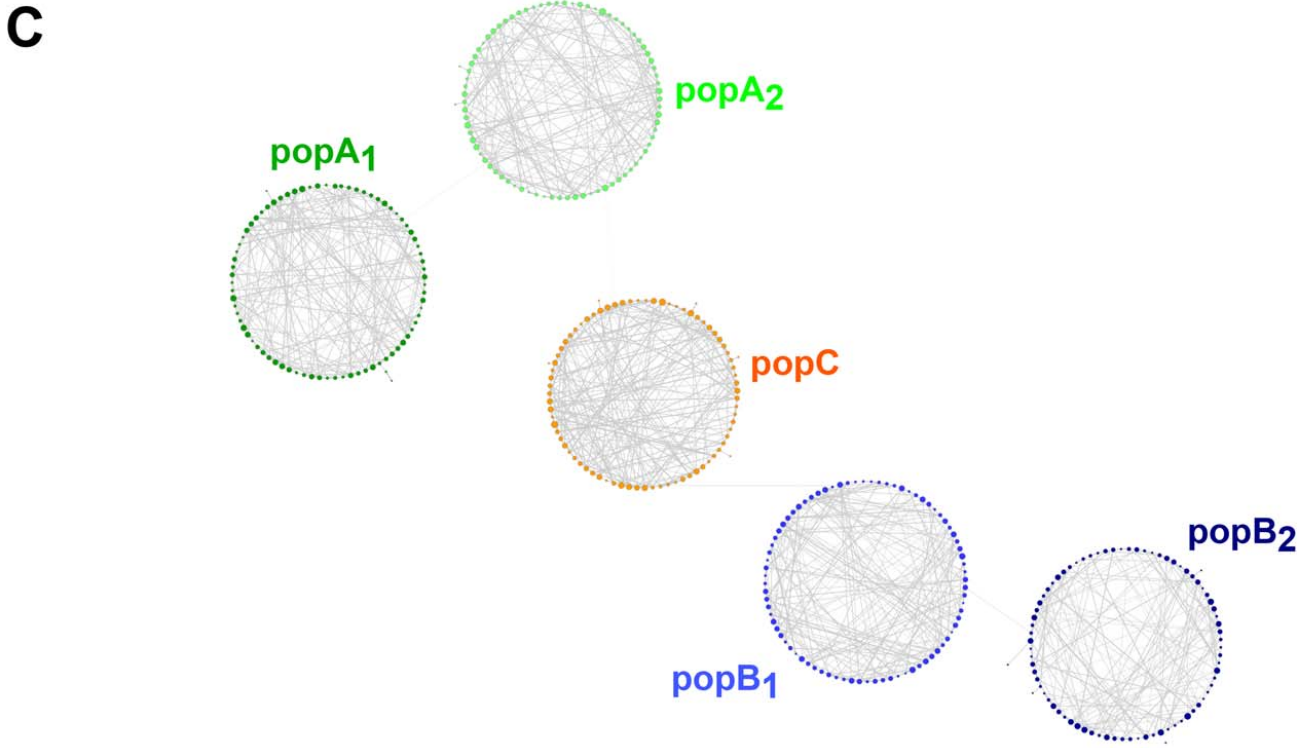
\includegraphics[width=1\linewidth,keepaspectratio]{../Figures/fig6c.png}
  \caption{Visualization of SPC clusters. Edges correspond to genetic
    similarity in the population distance matrix, and the sizes of nodes
    indicate its degree centrality. Nearby clusters are more related than
    distant ones\cite{neuditschko_netview:_2012}.}
\end{figure}

Like other network-based methods, the graphical structure of the output makes
it easy to visualize outliers and strongly divergent data, and the analysis can
then be adjusted accordingly. Also, the method preserves the structure of
genetic relationships within each cluster that is amenable to other network
analyses, such as centrality and modularity, though the values will require an
underlying population genetic theory to make them interpretable.

\subsection{Strength of Association (SA)}

Strength of Association (SA) is another network-based method that finds
communities of similar individuals given genetic
data~\cite{greenbaum_inference_2016}. It differs from Population Graphs in that
it computes community detection and partitions of genetic data, given an
arbitrary distance metric, rather than rely on conditional independence of
demes by approximating the data as derived from a multivariate Gaussian. SA is
fully non-parametric.

The null assumption of the model is that for a given dataset, there is no
subclustering, i.e.\ that all individuals follow a distribution where they are
expected to be equally distant from a population centroid defined by all the
genetic data. Networks where there is high inter-relatedness among individuals
violate this model, and these individuals can be compartmentalized into
modules, or communities, where the interconnectedness within the community is
higher for all individuals than interconnectedness outside of it. In network
terminology, the method produces a partition that maximizes the modularity of
all the communities, and its significance is measured by the extent to which it
deviates from the null network model. Many efficient methods for computing
communities exist~\cite{newman_modularity_2006}, and the significance of each
module is computed with permutation tests. Due to the vastness of genotype
data, the permutations are done on the edges of the graph rather then on the
data themselves.

The metric used to compute the interrelatedness can be any measure of genetic
similarity, but the authors for their own analysis select one that weights
connections based on the proportion of \textit{rare} shared variants. Measures
that are above an arbitrary threshold will be represented as edges in the
network, and those below will be dropped. The choice of threshold must be
chosen on a per-graph basis so that the overall network is not so dense that
modules are impossible to partition and not so sparse that
the network becomes too fragmented for analysis.

\begin{figure}
  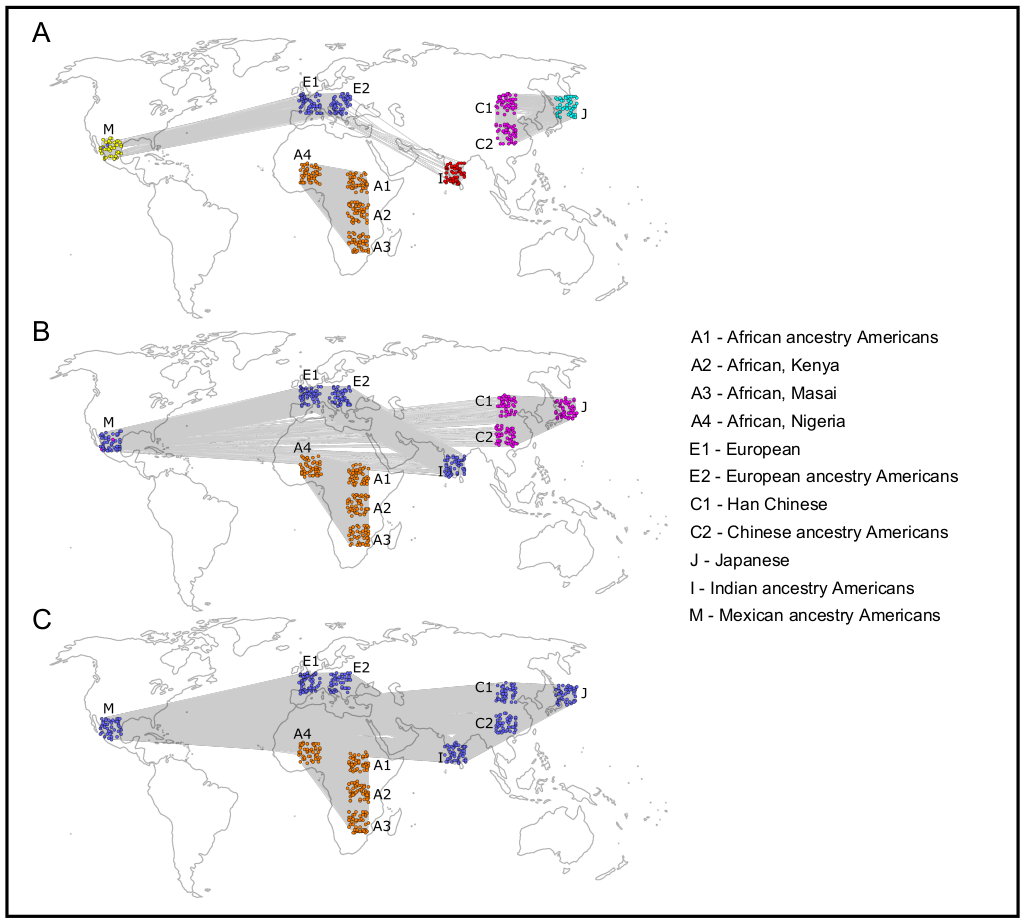
\includegraphics[width=1\linewidth,keepaspectratio]{../Figures/fig11.png}
  \caption{Clustering based on three different thresholds for the genetic
  relatedness: (A) high = 0.207 (Asia), 0.198; (B) medium = 0.194; (C) low =
  0.188~\cite{greenbaum_inference_2016}.}
\end{figure}

Once a meaningful graph partition is found, one then computes the Strength of
Association for each individual $i$:

\begin{align}
  SA(C, i) = \min_{k, C_k(i) \neq C} (Q_C - Q_{C_{{k}(i)}})
\end{align}

where $Q_C$ is the modularity of partition $C$ and $Q_{C_{{k}(i)}}$ is the
modularity of the partition where individual $i$ is removed and assigned to
community $k$ instead. The higher the value, the stronger an individual $i$ is
bound with its community.

All the SA values for a particular set of individuals and a community partition
form a Strength of Association Distribution (SAD). The dispersion around the
distribution has important implications regarding the demographic histories of
the represented populations. Large spread means that in each community, there
are many individuals that are less strongly `bound' to the community. It shares
variants with other communities and likely is evidence of admixture between
populations. Conversely, a very tight distribution suggests very little
admixture in individuals' evolutionary histories.

\begin{figure}
  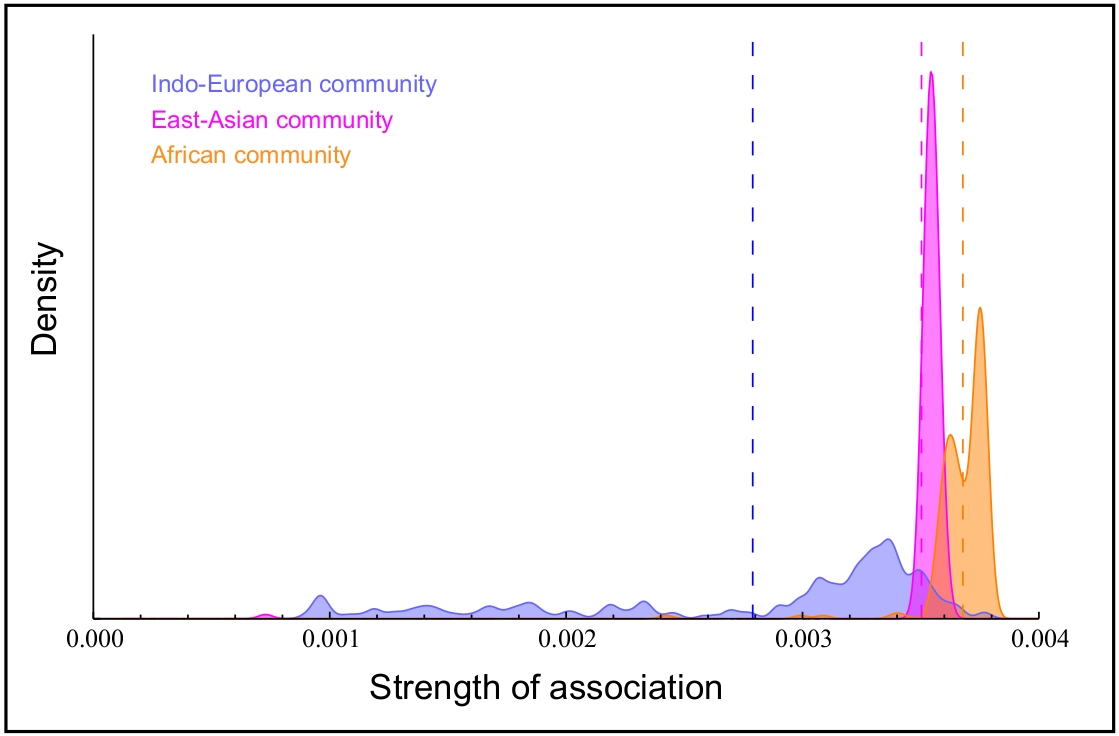
\includegraphics[width=1\linewidth,keepaspectratio]{../Figures/fig12.png}
  \caption{SAD distributions for human HapMap data. Dashed lines are mean SAD
  for each community~\cite{greenbaum_inference_2016}.}
\end{figure}

The method has been demonstrated to be able to differentiate populations that
model-based approaches are unable to do, specifically STRUCTURE with regard to
separating Chinese and Japanese HapMap data~\cite{newman_modularity_2006}. It
can also identify hybrid individuals given a set of known populations.

\section{Conclusions}

Network-based methods are an effective option for studying gene flow between
populations. They serve as an alternative to model-based ones in that they are
non-parametric --- they impose no prior assumptions on the structure of the
data that will affect the results of the analysis. Network-based methods are
also an alternative to PCA/MDS methods --- they are more flexible and can
better separate populations based on relevant genetic information. One can
define a genetic similarity matrix arbitrarily to form communities and
partitions that maximize the deviations between communities. This is in
contrast to PCA in that it relies on eigendecompositions that may not
necessarily produce information relevant to gene flow.

Whether one method is superior to another is context-dependent, and general
heuristic rules for when one should use one exclusively remain to be
discovered. Because the genetic networks themselves are highly complex and the
methods used to generate them non-parametric, this is a difficult problem. One
simply cannot evaluate the quality of such methods until the one sees the
results, and even then the reason why the methods work well or not are not
readily apparent. Indeed, network methods are often used in parallel with
others, where similarity in the results produced by one method buttresses
analysis done with another.

The flexibility and non-parametric nature of network methods they can be used
in a plethora of experimental situations, ranging from global human variation
to genotype variation across demes in local ecosystems. This strength, though,
is also a weakness when considering the interpretability of results. Network
methods are demonstrably able to outperform other methods in segregating
individuals~\cite{greenbaum_inference_2016,neuditschko_netview:_2012,dyer_population_2004},
but the exact meaning in terms of phenomena like strength of selection, loss of
heterozygosity due to drift, and so on are unclear. Model-based methods do not
have this limitation, and they can readily be augmented by developments in
population genetics and ecological theory. Though one can attempt circumvent
this by egressing network metrics against parameters in evolutionary or
ecological models, a well-defined, rigorous mathematical theory is necessary to
overcome it. Until then, network methods remain an excellent approach for
exploring analysis and visualizing the genetic relationships among individuals.

\newpage
\bibliography{publications}
\bibliographystyle{abbrv}

\end{document}
